\documentclass[1p]{elsarticle_modified}
%\bibliographystyle{elsarticle-num}

%\usepackage[colorlinks]{hyperref}
%\usepackage{abbrmath_seonhwa} %\Abb, \Ascr, \Acal ,\Abf, \Afrak
\usepackage{amsfonts}
\usepackage{amssymb}
\usepackage{amsmath}
\usepackage{amsthm}
\usepackage{scalefnt}
\usepackage{amsbsy}
\usepackage{kotex}
\usepackage{caption}
\usepackage{subfig}
\usepackage{color}
\usepackage{graphicx}
\usepackage{xcolor} %% white, black, red, green, blue, cyan, magenta, yellow
\usepackage{float}
\usepackage{setspace}
\usepackage{hyperref}

\usepackage{tikz}
\usetikzlibrary{arrows}

\usepackage{multirow}
\usepackage{array} % fixed length table
\usepackage{hhline}

%%%%%%%%%%%%%%%%%%%%%
\makeatletter
\renewcommand*\env@matrix[1][\arraystretch]{%
	\edef\arraystretch{#1}%
	\hskip -\arraycolsep
	\let\@ifnextchar\new@ifnextchar
	\array{*\c@MaxMatrixCols c}}
\makeatother %https://tex.stackexchange.com/questions/14071/how-can-i-increase-the-line-spacing-in-a-matrix
%%%%%%%%%%%%%%%

\usepackage[normalem]{ulem}

\newcommand{\msout}[1]{\ifmmode\text{\sout{\ensuremath{#1}}}\else\sout{#1}\fi}
%SOURCE: \msout is \stkout macro in https://tex.stackexchange.com/questions/20609/strikeout-in-math-mode

\newcommand{\cancel}[1]{
	\ifmmode
	{\color{red}\msout{#1}}
	\else
	{\color{red}\sout{#1}}
	\fi
}

\newcommand{\add}[1]{
	{\color{blue}\uwave{#1}}
}

\newcommand{\replace}[2]{
	\ifmmode
	{\color{red}\msout{#1}}{\color{blue}\uwave{#2}}
	\else
	{\color{red}\sout{#1}}{\color{blue}\uwave{#2}}
	\fi
}

\newcommand{\Sol}{\mathcal{S}} %segment
\newcommand{\D}{D} %diagram
\newcommand{\A}{\mathcal{A}} %arc


%%%%%%%%%%%%%%%%%%%%%%%%%%%%%5 test

\def\sl{\operatorname{\textup{SL}}(2,\Cbb)}
\def\psl{\operatorname{\textup{PSL}}(2,\Cbb)}
\def\quan{\mkern 1mu \triangleright \mkern 1mu}

\theoremstyle{definition}
\newtheorem{thm}{Theorem}[section]
\newtheorem{prop}[thm]{Proposition}
\newtheorem{lem}[thm]{Lemma}
\newtheorem{ques}[thm]{Question}
\newtheorem{cor}[thm]{Corollary}
\newtheorem{defn}[thm]{Definition}
\newtheorem{exam}[thm]{Example}
\newtheorem{rmk}[thm]{Remark}
\newtheorem{alg}[thm]{Algorithm}

\newcommand{\I}{\sqrt{-1}}
\begin{document}

%\begin{frontmatter}
%
%\title{Boundary parabolic representations of knots up to 8 crossings}
%
%%% Group authors per affiliation:
%\author{Yunhi Cho} 
%\address{Department of Mathematics, University of Seoul, Seoul, Korea}
%\ead{yhcho@uos.ac.kr}
%
%
%\author{Seonhwa Kim} %\fnref{s_kim}}
%\address{Center for Geometry and Physics, Institute for Basic Science, Pohang, 37673, Korea}
%\ead{ryeona17@ibs.re.kr}
%
%\author{Hyuk Kim}
%\address{Department of Mathematical Sciences, Seoul National University, Seoul 08826, Korea}
%\ead{hyukkim@snu.ac.kr}
%
%\author{Seokbeom Yoon}
%\address{Department of Mathematical Sciences, Seoul National University, Seoul, 08826,  Korea}
%\ead{sbyoon15@snu.ac.kr}
%
%\begin{abstract}
%We find all boundary parabolic representation of knots up to 8 crossings.
%
%\end{abstract}
%\begin{keyword}
%    \MSC[2010] 57M25 
%\end{keyword}
%
%\end{frontmatter}

%\linenumbers
%\tableofcontents
%
\newcommand\colored[1]{\textcolor{white}{\rule[-0.35ex]{0.8em}{1.4ex}}\kern-0.8em\color{red} #1}%
%\newcommand\colored[1]{\textcolor{white}{ #1}\kern-2.17ex	\textcolor{white}{ #1}\kern-1.81ex	\textcolor{white}{ #1}\kern-2.15ex\color{red}#1	}

{\Large $\underline{11a_{9}~(K11a_{9})}$}

\setlength{\tabcolsep}{10pt}
\renewcommand{\arraystretch}{1.6}
\vspace{1cm}\begin{tabular}{m{100pt}>{\centering\arraybackslash}m{274pt}}
\multirow{5}{120pt}{
	\centering
	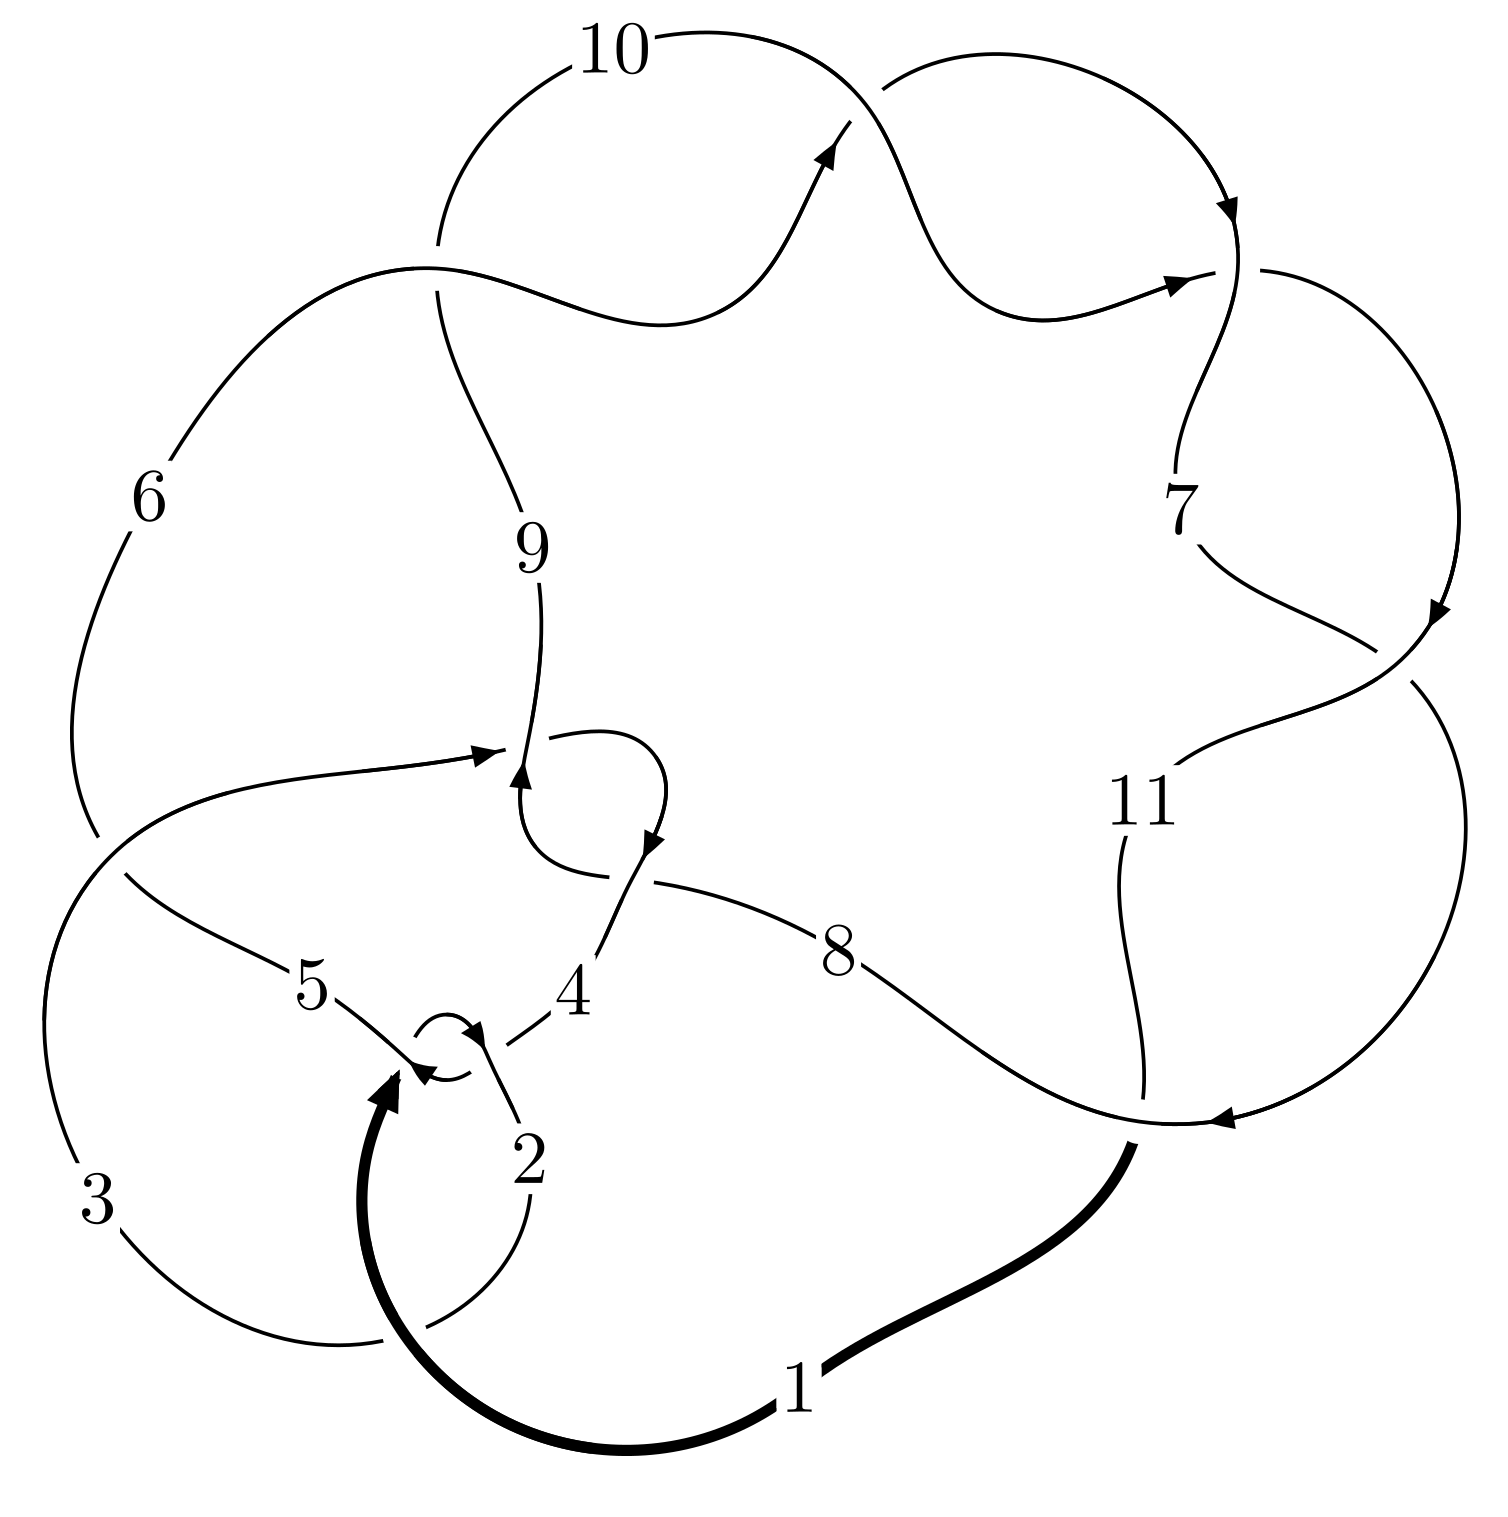
\includegraphics[width=112pt]{../../../GIT/diagram.site/Diagrams/png/258_11a_9.png}\\
\ \ \ A knot diagram\footnotemark}&
\allowdisplaybreaks
\textbf{Linearized knot diagam} \\
\cline{2-2}
 &
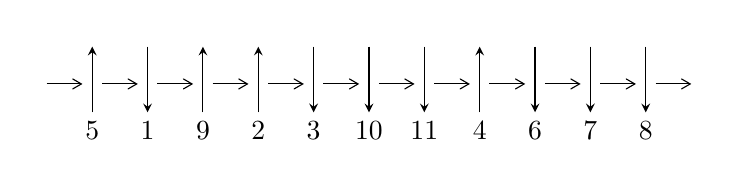
\begin{tikzpicture}[x=20pt, y=17pt]
	% nodes
	\node (C0) at (0, 0) {};
	\node (C1) at (1, 0) {};
	\node (C1U) at (1, +1) {};
	\node (C1D) at (1, -1) {5};

	\node (C2) at (2, 0) {};
	\node (C2U) at (2, +1) {};
	\node (C2D) at (2, -1) {1};

	\node (C3) at (3, 0) {};
	\node (C3U) at (3, +1) {};
	\node (C3D) at (3, -1) {9};

	\node (C4) at (4, 0) {};
	\node (C4U) at (4, +1) {};
	\node (C4D) at (4, -1) {2};

	\node (C5) at (5, 0) {};
	\node (C5U) at (5, +1) {};
	\node (C5D) at (5, -1) {3};

	\node (C6) at (6, 0) {};
	\node (C6U) at (6, +1) {};
	\node (C6D) at (6, -1) {10};

	\node (C7) at (7, 0) {};
	\node (C7U) at (7, +1) {};
	\node (C7D) at (7, -1) {11};

	\node (C8) at (8, 0) {};
	\node (C8U) at (8, +1) {};
	\node (C8D) at (8, -1) {4};

	\node (C9) at (9, 0) {};
	\node (C9U) at (9, +1) {};
	\node (C9D) at (9, -1) {6};

	\node (C10) at (10, 0) {};
	\node (C10U) at (10, +1) {};
	\node (C10D) at (10, -1) {7};

	\node (C11) at (11, 0) {};
	\node (C11U) at (11, +1) {};
	\node (C11D) at (11, -1) {8};
	\node (C12) at (12, 0) {};

	% arrows
	\draw[->,>={angle 60}]
	(C0) edge (C1) (C1) edge (C2) (C2) edge (C3) (C3) edge (C4) (C4) edge (C5) (C5) edge (C6) (C6) edge (C7) (C7) edge (C8) (C8) edge (C9) (C9) edge (C10) (C10) edge (C11) (C11) edge (C12) ;	\draw[->,>=stealth]
	(C1D) edge (C1U) (C2U) edge (C2D) (C3D) edge (C3U) (C4D) edge (C4U) (C5U) edge (C5D) (C6U) edge (C6D) (C7U) edge (C7D) (C8D) edge (C8U) (C9U) edge (C9D) (C10U) edge (C10D) (C11U) edge (C11D) ;
	\end{tikzpicture} \\
\hhline{~~} \\& 
\textbf{Solving Sequence} \\ \cline{2-2} 
 &
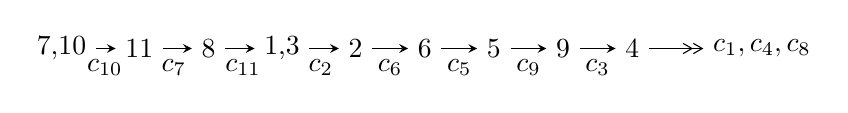
\begin{tikzpicture}[x=25pt, y=7pt]
	% node
	\node (A0) at (-1/8, 0) {7,10};
	\node (A1) at (1, 0) {11};
	\node (A2) at (2, 0) {8};
	\node (A3) at (49/16, 0) {1,3};
	\node (A4) at (33/8, 0) {2};
	\node (A5) at (41/8, 0) {6};
	\node (A6) at (49/8, 0) {5};
	\node (A7) at (57/8, 0) {9};
	\node (A8) at (65/8, 0) {4};
	\node (C1) at (1/2, -1) {$c_{10}$};
	\node (C2) at (3/2, -1) {$c_{7}$};
	\node (C3) at (5/2, -1) {$c_{11}$};
	\node (C4) at (29/8, -1) {$c_{2}$};
	\node (C5) at (37/8, -1) {$c_{6}$};
	\node (C6) at (45/8, -1) {$c_{5}$};
	\node (C7) at (53/8, -1) {$c_{9}$};
	\node (C8) at (61/8, -1) {$c_{3}$};
	\node (A9) at (10, 0) {$c_{1},c_{4},c_{8}$};

	% edge
	\draw[->,>=stealth]	
	(A0) edge (A1) (A1) edge (A2) (A2) edge (A3) (A3) edge (A4) (A4) edge (A5) (A5) edge (A6) (A6) edge (A7) (A7) edge (A8) ;
	\draw[->>,>={angle 60}]	
	(A8) edge (A9);
\end{tikzpicture} \\ 

\end{tabular} \\

\footnotetext{
The image of knot diagram is generated by the software ``\textbf{Draw programme}" developed by Andrew Bartholomew(\url{http://www.layer8.co.uk/maths/draw/index.htm\#Running-draw}), where we modified some parts for our purpose(\url{https://github.com/CATsTAILs/LinksPainter}).
}\phantom \\ \newline 
\centering \textbf{Ideals for irreducible components\footnotemark of $X_{\text{par}}$} 
 
\begin{align*}
I^u_{1}&=\langle 
u^{35}+u^{34}+\cdots+2 b-1,\;3 u^{35}+4 u^{34}+\cdots+2 a-2,\;u^{36}+3 u^{35}+\cdots-3 u^2-1\rangle \\
I^u_{2}&=\langle 
- a u+b,\;a^2+a+1,\;u^2- u-1\rangle \\
\\
\end{align*}
\raggedright * 2 irreducible components of $\dim_{\mathbb{C}}=0$, with total 40 representations.\\
\footnotetext{All coefficients of polynomials are rational numbers. But the coefficients are sometimes approximated in decimal forms when there is not enough margin.}
\newpage
\renewcommand{\arraystretch}{1}
\centering \section*{I. $I^u_{1}= \langle u^{35}+u^{34}+\cdots+2 b-1,\;3 u^{35}+4 u^{34}+\cdots+2 a-2,\;u^{36}+3 u^{35}+\cdots-3 u^2-1 \rangle$}
\flushleft \textbf{(i) Arc colorings}\\
\begin{tabular}{m{7pt} m{180pt} m{7pt} m{180pt} }
\flushright $a_{7}=$&$\begin{pmatrix}0\\u\end{pmatrix}$ \\
\flushright $a_{10}=$&$\begin{pmatrix}1\\0\end{pmatrix}$ \\
\flushright $a_{11}=$&$\begin{pmatrix}1\\u^2\end{pmatrix}$ \\
\flushright $a_{8}=$&$\begin{pmatrix}- u\\- u^3+u\end{pmatrix}$ \\
\flushright $a_{1}=$&$\begin{pmatrix}- u^2+1\\- u^4+2 u^2\end{pmatrix}$ \\
\flushright $a_{3}=$&$\begin{pmatrix}-\frac{3}{2} u^{35}-2 u^{34}+\cdots-\frac{5}{2} u+1\\-\frac{1}{2} u^{35}-\frac{1}{2} u^{34}+\cdots+4 u^2+\frac{1}{2}\end{pmatrix}$ \\
\flushright $a_{2}=$&$\begin{pmatrix}5 u^{35}+\frac{13}{2} u^{34}+\cdots+\frac{1}{2} u-\frac{5}{2}\\8 u^{35}+10 u^{34}+\cdots+3 u-5\end{pmatrix}$ \\
\flushright $a_{6}=$&$\begin{pmatrix}u\\u\end{pmatrix}$ \\
\flushright $a_{5}=$&$\begin{pmatrix}-\frac{1}{2} u^{35}- u^{34}+\cdots+\frac{11}{2} u+1\\-\frac{1}{2} u^{35}-\frac{1}{2} u^{34}+\cdots-2 u^2+\frac{1}{2}\end{pmatrix}$ \\
\flushright $a_{9}=$&$\begin{pmatrix}- u^2+1\\- u^2\end{pmatrix}$ \\
\flushright $a_{4}=$&$\begin{pmatrix}\frac{11}{2} u^{35}+7 u^{34}+\cdots-\frac{1}{2} u-3\\\frac{19}{2} u^{35}+\frac{23}{2} u^{34}+\cdots+3 u-\frac{11}{2}\end{pmatrix}$\\ \flushright $a_{4}=$&$\begin{pmatrix}\frac{11}{2} u^{35}+7 u^{34}+\cdots-\frac{1}{2} u-3\\\frac{19}{2} u^{35}+\frac{23}{2} u^{34}+\cdots+3 u-\frac{11}{2}\end{pmatrix}$\\&\end{tabular}
\flushleft \textbf{(ii) Obstruction class $= -1$}\\~\\
\flushleft \textbf{(iii) Cusp Shapes $= -\frac{5}{2} u^{35}-3 u^{34}+\cdots+\frac{23}{2} u^2+\frac{5}{2} u$}\\~\\
\newpage\renewcommand{\arraystretch}{1}
\flushleft \textbf{(iv) u-Polynomials at the component}\newline \\
\begin{tabular}{m{50pt}|m{274pt}}
Crossings & \hspace{64pt}u-Polynomials at each crossing \\
\hline $$\begin{aligned}c_{1},c_{4}\end{aligned}$$&$\begin{aligned}
&u^{36}+3 u^{35}+\cdots+2 u+1
\end{aligned}$\\
\hline $$\begin{aligned}c_{2}\end{aligned}$$&$\begin{aligned}
&u^{36}+19 u^{35}+\cdots+2 u+1
\end{aligned}$\\
\hline $$\begin{aligned}c_{3},c_{8}\end{aligned}$$&$\begin{aligned}
&u^{36}+u^{35}+\cdots-32 u-16
\end{aligned}$\\
\hline $$\begin{aligned}c_{5}\end{aligned}$$&$\begin{aligned}
&u^{36}-3 u^{35}+\cdots-156 u+41
\end{aligned}$\\
\hline $$\begin{aligned}c_{6},c_{7},c_{9}\\c_{10},c_{11}\end{aligned}$$&$\begin{aligned}
&u^{36}+3 u^{35}+\cdots-3 u^2-1
\end{aligned}$\\
\hline
\end{tabular}\\~\\
\newpage\renewcommand{\arraystretch}{1}
\flushleft \textbf{(v) Riley Polynomials at the component}\newline \\
\begin{tabular}{m{50pt}|m{274pt}}
Crossings & \hspace{64pt}Riley Polynomials at each crossing \\
\hline $$\begin{aligned}c_{1},c_{4}\end{aligned}$$&$\begin{aligned}
&y^{36}+19 y^{35}+\cdots+2 y+1
\end{aligned}$\\
\hline $$\begin{aligned}c_{2}\end{aligned}$$&$\begin{aligned}
&y^{36}- y^{35}+\cdots-46 y+1
\end{aligned}$\\
\hline $$\begin{aligned}c_{3},c_{8}\end{aligned}$$&$\begin{aligned}
&y^{36}+25 y^{35}+\cdots+896 y+256
\end{aligned}$\\
\hline $$\begin{aligned}c_{5}\end{aligned}$$&$\begin{aligned}
&y^{36}-21 y^{35}+\cdots+12482 y+1681
\end{aligned}$\\
\hline $$\begin{aligned}c_{6},c_{7},c_{9}\\c_{10},c_{11}\end{aligned}$$&$\begin{aligned}
&y^{36}-49 y^{35}+\cdots+6 y+1
\end{aligned}$\\
\hline
\end{tabular}\\~\\
\newpage\flushleft \textbf{(vi) Complex Volumes and Cusp Shapes}
$$\begin{array}{c|c|c}  
\text{Solutions to }I^u_{1}& \I (\text{vol} + \sqrt{-1}CS) & \text{Cusp shape}\\
 \hline 
\begin{aligned}
u &= -1.025520 + 0.116463 I \\
a &= -1.031170 + 0.432608 I \\
b &= -2.09741 + 0.72386 I\end{aligned}
 & -4.16025 + 3.63915 I & -10.15018 - 4.27650 I \\ \hline\begin{aligned}
u &= -1.025520 - 0.116463 I \\
a &= -1.031170 - 0.432608 I \\
b &= -2.09741 - 0.72386 I\end{aligned}
 & -4.16025 - 3.63915 I & -10.15018 + 4.27650 I \\ \hline\begin{aligned}
u &= \phantom{-}0.917325 + 0.063901 I \\
a &= -0.133059 - 1.056750 I \\
b &= \phantom{-}0.317589 + 0.408768 I\end{aligned}
 & -2.00047 - 2.57631 I & -10.63302 + 4.45192 I \\ \hline\begin{aligned}
u &= \phantom{-}0.917325 - 0.063901 I \\
a &= -0.133059 + 1.056750 I \\
b &= \phantom{-}0.317589 - 0.408768 I\end{aligned}
 & -2.00047 + 2.57631 I & -10.63302 - 4.45192 I \\ \hline\begin{aligned}
u &= \phantom{-}1.065990 + 0.299185 I \\
a &= \phantom{-}0.322094 - 0.440855 I \\
b &= \phantom{-}1.56593 - 0.19350 I\end{aligned}
 & -5.13782 - 4.39791 I & -8.11131 + 3.98843 I \\ \hline\begin{aligned}
u &= \phantom{-}1.065990 - 0.299185 I \\
a &= \phantom{-}0.322094 + 0.440855 I \\
b &= \phantom{-}1.56593 + 0.19350 I\end{aligned}
 & -5.13782 + 4.39791 I & -8.11131 - 3.98843 I \\ \hline\begin{aligned}
u &= \phantom{-}1.082360 + 0.370781 I \\
a &= -0.558691 + 0.183985 I \\
b &= -2.00888 + 0.15748 I\end{aligned}
 & -8.00799 - 9.41273 I & -10.73207 + 7.33022 I \\ \hline\begin{aligned}
u &= \phantom{-}1.082360 - 0.370781 I \\
a &= -0.558691 - 0.183985 I \\
b &= -2.00888 - 0.15748 I\end{aligned}
 & -8.00799 + 9.41273 I & -10.73207 - 7.33022 I \\ \hline\begin{aligned}
u &= -0.852163\phantom{ +0.000000I} \\
a &= \phantom{-}0.572389\phantom{ +0.000000I} \\
b &= \phantom{-}1.20255\phantom{ +0.000000I}\end{aligned}
 & -1.51344\phantom{ +0.000000I} & -5.97070\phantom{ +0.000000I} \\ \hline\begin{aligned}
u &= \phantom{-}1.178870 + 0.253014 I \\
a &= -0.540902 + 0.868497 I \\
b &= -1.39570 + 0.91291 I\end{aligned}
 & -9.53106 - 0.77090 I & -13.03537 + 0.66876 I\\
 \hline 
 \end{array}$$\newpage$$\begin{array}{c|c|c}  
\text{Solutions to }I^u_{1}& \I (\text{vol} + \sqrt{-1}CS) & \text{Cusp shape}\\
 \hline 
\begin{aligned}
u &= \phantom{-}1.178870 - 0.253014 I \\
a &= -0.540902 - 0.868497 I \\
b &= -1.39570 - 0.91291 I\end{aligned}
 & -9.53106 + 0.77090 I & -13.03537 - 0.66876 I \\ \hline\begin{aligned}
u &= -0.465838 + 0.569982 I \\
a &= -0.135891 - 0.713585 I \\
b &= \phantom{-}0.582474 + 0.680739 I\end{aligned}
 & -4.25762 - 2.03075 I & -9.39588 + 0.30706 I \\ \hline\begin{aligned}
u &= -0.465838 - 0.569982 I \\
a &= -0.135891 + 0.713585 I \\
b &= \phantom{-}0.582474 - 0.680739 I\end{aligned}
 & -4.25762 + 2.03075 I & -9.39588 - 0.30706 I \\ \hline\begin{aligned}
u &= -0.680312 + 0.218264 I \\
a &= \phantom{-}0.215818 - 0.256120 I \\
b &= \phantom{-}0.392517 - 0.767490 I\end{aligned}
 & -1.43730 + 0.46103 I & -9.15571 - 0.89205 I \\ \hline\begin{aligned}
u &= -0.680312 - 0.218264 I \\
a &= \phantom{-}0.215818 + 0.256120 I \\
b &= \phantom{-}0.392517 + 0.767490 I\end{aligned}
 & -1.43730 - 0.46103 I & -9.15571 + 0.89205 I \\ \hline\begin{aligned}
u &= -0.294050 + 0.635512 I \\
a &= -0.93728 - 1.18603 I \\
b &= \phantom{-}0.435962 + 0.264963 I\end{aligned}
 & -3.72424 + 5.98943 I & -7.50022 - 6.65502 I \\ \hline\begin{aligned}
u &= -0.294050 - 0.635512 I \\
a &= -0.93728 + 1.18603 I \\
b &= \phantom{-}0.435962 - 0.264963 I\end{aligned}
 & -3.72424 - 5.98943 I & -7.50022 + 6.65502 I \\ \hline\begin{aligned}
u &= -0.300828 + 0.511616 I \\
a &= \phantom{-}0.900271 + 0.580279 I \\
b &= -0.322840 - 0.451012 I\end{aligned}
 & -0.88449 + 1.61128 I & -3.96504 - 4.05315 I \\ \hline\begin{aligned}
u &= -0.300828 - 0.511616 I \\
a &= \phantom{-}0.900271 - 0.580279 I \\
b &= -0.322840 + 0.451012 I\end{aligned}
 & -0.88449 - 1.61128 I & -3.96504 + 4.05315 I \\ \hline\begin{aligned}
u &= \phantom{-}1.60354 + 0.03866 I \\
a &= -0.577687 - 1.062600 I \\
b &= -0.73772 - 1.35775 I\end{aligned}
 & -9.29333 - 1.36083 I & \phantom{-0.000000 } 0\\
 \hline 
 \end{array}$$\newpage$$\begin{array}{c|c|c}  
\text{Solutions to }I^u_{1}& \I (\text{vol} + \sqrt{-1}CS) & \text{Cusp shape}\\
 \hline 
\begin{aligned}
u &= \phantom{-}1.60354 - 0.03866 I \\
a &= -0.577687 + 1.062600 I \\
b &= -0.73772 + 1.35775 I\end{aligned}
 & -9.29333 + 1.36083 I & \phantom{-0.000000 } 0 \\ \hline\begin{aligned}
u &= \phantom{-}0.003501 + 0.334247 I \\
a &= \phantom{-}2.06412 - 0.29075 I \\
b &= -0.222553 - 0.457483 I\end{aligned}
 & \phantom{-}0.57956 + 1.37320 I & \phantom{-}1.27470 - 4.45868 I \\ \hline\begin{aligned}
u &= \phantom{-}0.003501 - 0.334247 I \\
a &= \phantom{-}2.06412 + 0.29075 I \\
b &= -0.222553 + 0.457483 I\end{aligned}
 & \phantom{-}0.57956 - 1.37320 I & \phantom{-}1.27470 + 4.45868 I \\ \hline\begin{aligned}
u &= \phantom{-}0.220883 + 0.210533 I \\
a &= -2.72148 + 0.23613 I \\
b &= \phantom{-}0.536583 + 0.437480 I\end{aligned}
 & -0.27564 - 2.47765 I & \phantom{-}1.24066 + 5.09366 I \\ \hline\begin{aligned}
u &= \phantom{-}0.220883 - 0.210533 I \\
a &= -2.72148 - 0.23613 I \\
b &= \phantom{-}0.536583 - 0.437480 I\end{aligned}
 & -0.27564 + 2.47765 I & \phantom{-}1.24066 - 5.09366 I \\ \hline\begin{aligned}
u &= \phantom{-}1.70560\phantom{ +0.000000I} \\
a &= -2.31988\phantom{ +0.000000I} \\
b &= -2.94838\phantom{ +0.000000I}\end{aligned}
 & -10.7808\phantom{ +0.000000I} & \phantom{-0.000000 } 0 \\ \hline\begin{aligned}
u &= -1.71389 + 0.01340 I \\
a &= -0.457517 + 0.775429 I \\
b &= -0.66586 + 1.78211 I\end{aligned}
 & -11.48460 + 2.85990 I & \phantom{-0.000000 } 0 \\ \hline\begin{aligned}
u &= -1.71389 - 0.01340 I \\
a &= -0.457517 - 0.775429 I \\
b &= -0.66586 - 1.78211 I\end{aligned}
 & -11.48460 - 2.85990 I & \phantom{-0.000000 } 0 \\ \hline\begin{aligned}
u &= \phantom{-}1.73373 + 0.02857 I \\
a &= \phantom{-}2.85868 + 0.56360 I \\
b &= \phantom{-}3.62671 + 0.70465 I\end{aligned}
 & -14.0947 - 4.2255 I & \phantom{-0.000000 } 0 \\ \hline\begin{aligned}
u &= \phantom{-}1.73373 - 0.02857 I \\
a &= \phantom{-}2.85868 - 0.56360 I \\
b &= \phantom{-}3.62671 - 0.70465 I\end{aligned}
 & -14.0947 + 4.2255 I & \phantom{-0.000000 } 0\\
 \hline 
 \end{array}$$\newpage$$\begin{array}{c|c|c}  
\text{Solutions to }I^u_{1}& \I (\text{vol} + \sqrt{-1}CS) & \text{Cusp shape}\\
 \hline 
\begin{aligned}
u &= -1.74040 + 0.07931 I \\
a &= -2.19385 - 0.26897 I \\
b &= -3.06657 + 0.17165 I\end{aligned}
 & -15.1592 + 5.9753 I & \phantom{-0.000000 } 0 \\ \hline\begin{aligned}
u &= -1.74040 - 0.07931 I \\
a &= -2.19385 + 0.26897 I \\
b &= -3.06657 - 0.17165 I\end{aligned}
 & -15.1592 - 5.9753 I & \phantom{-0.000000 } 0 \\ \hline\begin{aligned}
u &= -1.74533 + 0.09973 I \\
a &= \phantom{-}2.64626 + 0.43864 I \\
b &= \phantom{-}3.66599 + 0.11964 I\end{aligned}
 & -18.0669 + 11.3850 I & \phantom{-0.000000 } 0 \\ \hline\begin{aligned}
u &= -1.74533 - 0.09973 I \\
a &= \phantom{-}2.64626 - 0.43864 I \\
b &= \phantom{-}3.66599 - 0.11964 I\end{aligned}
 & -18.0669 - 11.3850 I & \phantom{-0.000000 } 0 \\ \hline\begin{aligned}
u &= -1.76676 + 0.06022 I \\
a &= \phantom{-}1.65403 + 0.87991 I \\
b &= \phantom{-}2.26669 + 0.61564 I\end{aligned}
 & \phantom{-}19.3219 + 2.0938 I & \phantom{-0.000000 } 0 \\ \hline\begin{aligned}
u &= -1.76676 - 0.06022 I \\
a &= \phantom{-}1.65403 - 0.87991 I \\
b &= \phantom{-}2.26669 - 0.61564 I\end{aligned}
 & \phantom{-}19.3219 - 2.0938 I & \phantom{-0.000000 } 0\\
 \hline 
 \end{array}$$\newpage\newpage\renewcommand{\arraystretch}{1}
\centering \section*{II. $I^u_{2}= \langle - a u+b,\;a^2+a+1,\;u^2- u-1 \rangle$}
\flushleft \textbf{(i) Arc colorings}\\
\begin{tabular}{m{7pt} m{180pt} m{7pt} m{180pt} }
\flushright $a_{7}=$&$\begin{pmatrix}0\\u\end{pmatrix}$ \\
\flushright $a_{10}=$&$\begin{pmatrix}1\\0\end{pmatrix}$ \\
\flushright $a_{11}=$&$\begin{pmatrix}1\\u+1\end{pmatrix}$ \\
\flushright $a_{8}=$&$\begin{pmatrix}- u\\- u-1\end{pmatrix}$ \\
\flushright $a_{1}=$&$\begin{pmatrix}- u\\- u\end{pmatrix}$ \\
\flushright $a_{3}=$&$\begin{pmatrix}a\\a u\end{pmatrix}$ \\
\flushright $a_{2}=$&$\begin{pmatrix}a u+a\\2 a u\end{pmatrix}$ \\
\flushright $a_{6}=$&$\begin{pmatrix}u\\u\end{pmatrix}$ \\
\flushright $a_{5}=$&$\begin{pmatrix}a+u+1\\a u+2 u\end{pmatrix}$ \\
\flushright $a_{9}=$&$\begin{pmatrix}- u\\- u-1\end{pmatrix}$ \\
\flushright $a_{4}=$&$\begin{pmatrix}a\\a u\end{pmatrix}$\\ \flushright $a_{4}=$&$\begin{pmatrix}a\\a u\end{pmatrix}$\\&\end{tabular}
\flushleft \textbf{(ii) Obstruction class $= 1$}\\~\\
\flushleft \textbf{(iii) Cusp Shapes $= -2 a u-3 a- u-8$}\\~\\
\newpage\renewcommand{\arraystretch}{1}
\flushleft \textbf{(iv) u-Polynomials at the component}\newline \\
\begin{tabular}{m{50pt}|m{274pt}}
Crossings & \hspace{64pt}u-Polynomials at each crossing \\
\hline $$\begin{aligned}c_{1},c_{2},c_{5}\end{aligned}$$&$\begin{aligned}
&(u^2+u+1)^2
\end{aligned}$\\
\hline $$\begin{aligned}c_{3},c_{8}\end{aligned}$$&$\begin{aligned}
&u^4
\end{aligned}$\\
\hline $$\begin{aligned}c_{4}\end{aligned}$$&$\begin{aligned}
&(u^2- u+1)^2
\end{aligned}$\\
\hline $$\begin{aligned}c_{6},c_{7}\end{aligned}$$&$\begin{aligned}
&(u^2+u-1)^2
\end{aligned}$\\
\hline $$\begin{aligned}c_{9},c_{10},c_{11}\end{aligned}$$&$\begin{aligned}
&(u^2- u-1)^2
\end{aligned}$\\
\hline
\end{tabular}\\~\\
\newpage\renewcommand{\arraystretch}{1}
\flushleft \textbf{(v) Riley Polynomials at the component}\newline \\
\begin{tabular}{m{50pt}|m{274pt}}
Crossings & \hspace{64pt}Riley Polynomials at each crossing \\
\hline $$\begin{aligned}c_{1},c_{2},c_{4}\\c_{5}\end{aligned}$$&$\begin{aligned}
&(y^2+y+1)^2
\end{aligned}$\\
\hline $$\begin{aligned}c_{3},c_{8}\end{aligned}$$&$\begin{aligned}
&y^4
\end{aligned}$\\
\hline $$\begin{aligned}c_{6},c_{7},c_{9}\\c_{10},c_{11}\end{aligned}$$&$\begin{aligned}
&(y^2-3 y+1)^2
\end{aligned}$\\
\hline
\end{tabular}\\~\\
\newpage\flushleft \textbf{(vi) Complex Volumes and Cusp Shapes}
$$\begin{array}{c|c|c}  
\text{Solutions to }I^u_{2}& \I (\text{vol} + \sqrt{-1}CS) & \text{Cusp shape}\\
 \hline 
\begin{aligned}
u &= -0.618034\phantom{ +0.000000I} \\
a &= -0.500000 + 0.866025 I \\
b &= \phantom{-}0.309017 - 0.535233 I\end{aligned}
 & -0.98696 + 2.02988 I & -6.50000 - 1.52761 I \\ \hline\begin{aligned}
u &= -0.618034\phantom{ +0.000000I} \\
a &= -0.500000 - 0.866025 I \\
b &= \phantom{-}0.309017 + 0.535233 I\end{aligned}
 & -0.98696 - 2.02988 I & -6.50000 + 1.52761 I \\ \hline\begin{aligned}
u &= \phantom{-}1.61803\phantom{ +0.000000I} \\
a &= -0.500000 + 0.866025 I \\
b &= -0.80902 + 1.40126 I\end{aligned}
 & -8.88264 + 2.02988 I & -6.50000 - 5.40059 I \\ \hline\begin{aligned}
u &= \phantom{-}1.61803\phantom{ +0.000000I} \\
a &= -0.500000 - 0.866025 I \\
b &= -0.80902 - 1.40126 I\end{aligned}
 & -8.88264 - 2.02988 I & -6.50000 + 5.40059 I\\
 \hline 
 \end{array}$$\newpage
\newpage\renewcommand{\arraystretch}{1}
\centering \section*{ III. u-Polynomials}
\begin{tabular}{m{50pt}|m{274pt}}
Crossings & \hspace{64pt}u-Polynomials at each crossing \\
\hline $$\begin{aligned}c_{1}\end{aligned}$$&$\begin{aligned}
&((u^2+u+1)^2)(u^{36}+3 u^{35}+\cdots+2 u+1)
\end{aligned}$\\
\hline $$\begin{aligned}c_{2}\end{aligned}$$&$\begin{aligned}
&((u^2+u+1)^2)(u^{36}+19 u^{35}+\cdots+2 u+1)
\end{aligned}$\\
\hline $$\begin{aligned}c_{3},c_{8}\end{aligned}$$&$\begin{aligned}
&u^4(u^{36}+u^{35}+\cdots-32 u-16)
\end{aligned}$\\
\hline $$\begin{aligned}c_{4}\end{aligned}$$&$\begin{aligned}
&((u^2- u+1)^2)(u^{36}+3 u^{35}+\cdots+2 u+1)
\end{aligned}$\\
\hline $$\begin{aligned}c_{5}\end{aligned}$$&$\begin{aligned}
&((u^2+u+1)^2)(u^{36}-3 u^{35}+\cdots-156 u+41)
\end{aligned}$\\
\hline $$\begin{aligned}c_{6},c_{7}\end{aligned}$$&$\begin{aligned}
&((u^2+u-1)^2)(u^{36}+3 u^{35}+\cdots-3 u^2-1)
\end{aligned}$\\
\hline $$\begin{aligned}c_{9},c_{10},c_{11}\end{aligned}$$&$\begin{aligned}
&((u^2- u-1)^2)(u^{36}+3 u^{35}+\cdots-3 u^2-1)
\end{aligned}$\\
\hline
\end{tabular}\newpage\renewcommand{\arraystretch}{1}
\centering \section*{ IV. Riley Polynomials}
\begin{tabular}{m{50pt}|m{274pt}}
Crossings & \hspace{64pt}Riley Polynomials at each crossing \\
\hline $$\begin{aligned}c_{1},c_{4}\end{aligned}$$&$\begin{aligned}
&((y^2+y+1)^2)(y^{36}+19 y^{35}+\cdots+2 y+1)
\end{aligned}$\\
\hline $$\begin{aligned}c_{2}\end{aligned}$$&$\begin{aligned}
&((y^2+y+1)^2)(y^{36}- y^{35}+\cdots-46 y+1)
\end{aligned}$\\
\hline $$\begin{aligned}c_{3},c_{8}\end{aligned}$$&$\begin{aligned}
&y^4(y^{36}+25 y^{35}+\cdots+896 y+256)
\end{aligned}$\\
\hline $$\begin{aligned}c_{5}\end{aligned}$$&$\begin{aligned}
&((y^2+y+1)^2)(y^{36}-21 y^{35}+\cdots+12482 y+1681)
\end{aligned}$\\
\hline $$\begin{aligned}c_{6},c_{7},c_{9}\\c_{10},c_{11}\end{aligned}$$&$\begin{aligned}
&((y^2-3 y+1)^2)(y^{36}-49 y^{35}+\cdots+6 y+1)
\end{aligned}$\\
\hline
\end{tabular}
\vskip 2pc
\end{document}